\section{DYNAMICAL ORIGINS OF OBSERVABLE MEMORY}
\label{sec:dynamics}

\subsection{Observable Forgetting}

An old input loses its influence if each new update shrinks differences
between earlier states.  Suppose every channel contracts trace distance
$D_{\rm tr}(\rho,\sigma)=\tfrac12\|\rho-\sigma\|_1$ by a uniform factor:
\begin{equation}
 D_{\rm tr}\!\left(\Phi_u(\rho),\Phi_u(\sigma)\right)
 \leq\eta D_{\rm tr}(\rho,\sigma),\qquad 0\leq\eta<1.
 \label{eq:incremental-channel}
\end{equation}
After $d$ common inputs, a scalar observable $O$ then obeys
\begin{equation}
 D_d\leq 2\|O\|_\infty\eta^d.
 \label{eq:contraction-bound}
\end{equation}
Old-state influence therefore falls exponentially, making finite context
sufficient for any fixed information-error tolerance.

The entire state need not forget.  Only differences that old inputs can
create and declared outputs can reveal matter.  Unreachable differences
cannot encode an input distinction; permanently invisible differences
cannot obstruct emulation.  Visibility must include future outputs, because
later inputs may reveal a currently hidden difference.

Restricting to the span of reachable differences and identifying those
indistinguishable under every future input gives the
\emph{reachable-observable quotient}.  Each channel induces a linear update
$A_u$ on this space.  Their joint spectral radius tests the long-term
damping over all input sequences:
\begin{equation}
 r_{\rm vis}
 =\lim_{d\to\infty}
 \sup_{u_1,\ldots,u_d}
 \|A_{u_d}\cdots A_{u_1}\|^{1/d}.
 \label{eq:visible-radius-definition}
\end{equation}
It measures the slowest asymptotic damping over allowed input sequences and
does not depend on the norm used.  The Appendix gives the quotient
construction and its norm properties
\cite{rota1960joint,jungers2009joint}.

\textit{Observable-memory theorem.}  For finite-dimensional QRCs with a
compact input alphabet, input-continuous channels, a fixed finite observable
output vector, and freely concatenable suffixes, the reachable-observable
joint spectral radius satisfies
\begin{equation}
 D_d\to0\quad\Longleftrightarrow\quad r_{\rm vis}<1,
 \qquad
 \lim_{d\to\infty}D_d^{1/d}=r_{\rm vis}.
 \label{eq:visible-memory-theorem}
\end{equation}
The missing past becomes uniformly negligible exactly when all relevant
state differences are uniformly damped.  The Appendix proves this by
comparing $D_d$ with the largest length-$d$ update product up to fixed
factors.  Individual-channel spectra do not suffice: a suffix can contain
arbitrary channel products.  Full-state contraction is unnecessary because
unreachable and permanently invisible directions have been removed.

This criterion also determines how much explicit context is needed.
For scalar output, let
\begin{equation}
 d_\varepsilon=\min\{d:D_d<2\varepsilon\}
 \label{eq:context-length}
\end{equation}
be the shortest window for which some unrestricted predictor has worst-case
error below $\varepsilon$.  When $0<r_{\rm vis}<1$,
\begin{equation}
 \lim_{\varepsilon\downarrow0}
 \frac{d_\varepsilon}{\log(1/\varepsilon)}
 =\frac{1}{-\log r_{\rm vis}}.
 \label{eq:window-complexity}
\end{equation}
Slowly fading observable memory therefore requires a long explicit context.
This law concerns the information requirement, not the feature or training
cost of a QELM.  Under full-state contraction,
$r_{\rm vis}\leq\eta<1$; the next construction realizes the opposite
boundary, $r_{\rm vis}=1$.

% Queue the resource figure for the experiments page without a late float gap.
\begin{figure*}[t]
 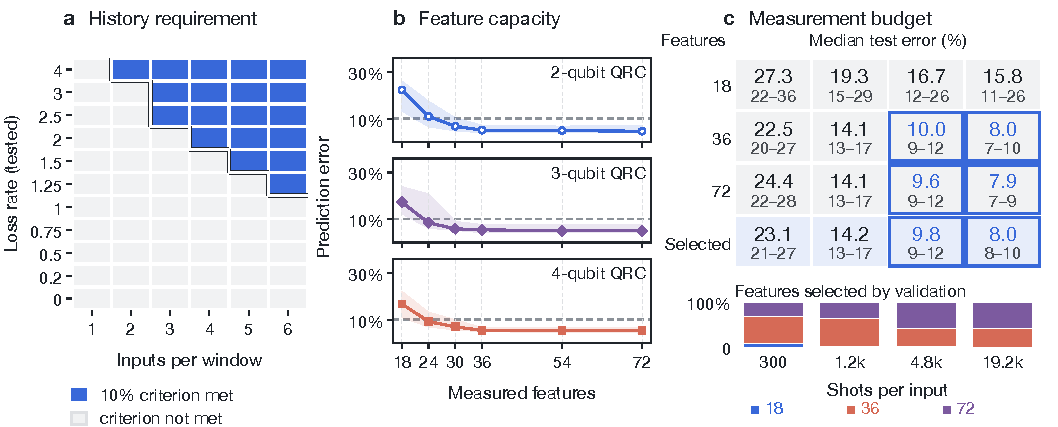
\includegraphics[width=\textwidth]{fig03_resource_diagnosis.pdf}
 \caption{Three resources address three limits.  Errors are NRMSE percentages;
 dashed lines mark $10\%=0.10$.  a,b Two- and three-qubit targets:
 a Old-history error versus scaled context $\gamma_T\Delta t\,d$.
 b Total QELM error versus features at $\gamma_T=4,d=6$, where history is
 sufficient. Curves show size-wise root medians; whiskers span the
 10th--90th root percentiles, describing variability rather than confidence
 intervals.
 c Validation-selected test error versus shots, with root medians and the
 selected policy's 10th--90th percentile whiskers. This post-confirmatory
 four-qubit follow-up repeats complete fitting and selection 16 times per root.}
 \label{fig:resource-diagnosis}
\end{figure*}

\subsection{Protected Memory}

Two qubits provide a write--protect--read example.  An old local pulse
changes the population of the antisymmetric singlet state.  Subsequent
symmetric drives and collective loss preserve it.  Pauli correlations
reveal the difference after the old input has left the window.  The singlet
projector is
\begin{equation}
 P_-=|\psi^-\rangle\!\langle\psi^-|
 =\frac{II-XX-YY-ZZ}{4},
 \label{eq:protected-singlet}
\end{equation}
so its expectation can be recovered from $XX$, $YY$, and $ZZ$ measurements.

Every update uses the same time-homogeneous input alphabet $a=(u,q)$.
Here $u$ controls the symmetric drive and the flag $q$ permits an
addressable pulse on the first qubit.  Two histories differ only in an old
flagged input; afterward they receive the same sequence from the freely
iterable $q=0$ subalphabet.  For that sequence, the population difference
is conserved.  The Appendix gives the pulse calculation and exact gap;
the full channel and control parameters appear in the Appendix.

More generally, suppose two reachable states differ by $\delta>0$ in the
expectation of an operator $P$, and a nonempty suffix subalphabet can be
iterated freely after both histories.  If
$\Phi_u^\dagger(P)=P$ for each symbol in that subalphabet, every such suffix
preserves the difference.  With the declared scalar output
$Y=\operatorname{Tr}(P\rho)$,
\begin{equation}
 D_d\geq\delta\qquad\text{for every finite }d.
 \label{eq:protected-mode}
\end{equation}
Equation~\eqref{eq:window-law} then forces worst-case absolute error of at
least $\delta/2$ for every finite-window emulator.  The singlet construction
supplies one process and one trajectory pair for every window length,
giving $r_{\rm vis}=1$ in Eq.~\eqref{eq:visible-memory-theorem}.

Matched controls distinguish protection from slow decay: local loss reduces
the gap, while asymmetric collective loss breaks exact conservation without
necessarily causing rapid erasure.  The storage mechanism is quantum; the
information bound applies to both quantum and classical stateless window
models.  When this obstruction is absent, emulation still needs sufficient
features and measurement precision.
